\documentclass[14pt, a4paper]{extarticle}
% Русская локализация
\usepackage[english,russian]{babel}


\usepackage{appendix}
\usepackage{alphabeta}

% Использование математических шрифтов
\usepackage{unicode-math}

% Шрифты
\usepackage{fontspec}
\usepackage{courier}
\defaultfontfeatures{Ligatures={TeX},Renderer=Basic}
\setmainfont[Ligatures={TeX}]{Times New Roman}
\setmonofont{Courier New}
\setmathfont{XITS Math}

% Расширенные ссылки
\usepackage{nameref}

% Оформление URL
\usepackage{xurl}
\usepackage{hyperref}
\hypersetup{
  colorlinks,
  citecolor=black,
  filecolor=black,
  linkcolor=black,
  urlcolor=black,
  breaklinks=true,
}
\urlstyle{same}

% Поддержка изображений
\usepackage{graphicx}
\graphicspath{{./images/}}
\DeclareGraphicsExtensions{.jpg,.png}
\usepackage{svg}

% Таблицы
\usepackage{tabularx}
\usepackage{tabulary}
\usepackage{ltablex}
\usepackage{multirow}
\usepackage{hhline}
% Выравнивание по левому краю, с многострочностью
\newcolumntype{s}{>{\raggedright\arraybackslash}X}

% Поддержка листингов
\usepackage{listings}
\lstdefinestyle{gost}{
  basicstyle=\ttfamily\footnotesize,
  breakatwhitespace=false,
  breaklines=true,
  keepspaces=true,
  showspaces=false,
  showstringspaces=false,
  frame=single
}
\lstset{style=gost}%

% Отступ первой строки первого абзаца
\usepackage{indentfirst}
\linespread{1.25}

% Размер полей в документе
\usepackage{geometry}
\geometry{left=3cm}
\geometry{right=1cm}
\geometry{top=2cm}
\geometry{bottom=2cm}

% Абзацный отступ
\setlength{\parindent}{1.25cm}

% Отступ для элементов в списке
\usepackage{enumitem}
\setlist{left=\parindent, labelsep=1cm, itemsep=0pt, topsep=0pt}

% Загрузка pdf-документов (нужно для титульных листов)
\usepackage[final]{pdfpages}
% Возможность поворота pdf файло
\usepackage{pdflscape}
\usepackage{everypage}

\newcommand{\Lpagenumber}{\ifdim\textwidth=\linewidth\else\bgroup%
    \dimendef\margin=0 %use \margin instead of \dimen0
    \ifodd\value{page}\margin=\oddsidemargin
    \else\margin=\evensidemargin%
    \fi

\raisebox{\dimexpr-\topmargin-\headheight-\headsep-0.5\linewidth}[0pt][0pt]{%
      \rlap{\hspace{\dimexpr-\margin+\textheight+\footskip}%
        \llap{\rotatebox{90}{\thepage}}}}%
    \egroup\fi}
\AddEverypageHook{\Lpagenumber}%

\usepackage{float}
% Форматирование подписей
\usepackage{caption}

\usepackage{newfloat}
% \DeclareCaptionType{listing}

\DeclareCaptionLabelSeparator{emdash}{\;\textemdash\;}
\captionsetup[figure]{name={Рисунок}, labelsep=emdash, justification=centering,
position=above, singlelinecheck=off, font={small, bf}, labelfont=bf, skip=6pt}
\captionsetup[table]{name={Таблица}, labelsep=emdash,
justification=raggedright, position=top, singlelinecheck=off, font={small, it},
labelfont=it, skip=6pt, margin=0cm}
% \captionsetup[lstlisting]{labelsep=emdash, justification=raggedright,
% position=top, singlelinecheck=off, font={small, it}, labelfont=it, skip=6pt,
% margin=0cm}

% Нумеровать внутри заголовков первого уровня
\counterwithin{figure}{section}
\counterwithin{table}{section}
% \counterwithin{lstlisting}{section}
\AtBeginDocument{\counterwithin{lstlisting}{section}}

% Отключение переносов текста
\usepackage{ragged2e}
\justifying
\tolerance=500
\hyphenpenalty=10000
\emergencystretch=3em

% Форматирование заголовков
\usepackage{titlesec}
% Оформление заголовка первого уровня
% Полужирное начертание
% Кегль 18 пт
% С новой страницы
\titleformat{\section}[block]
{\newpage\bfseries\fontsize{18pt}{21.6pt}\selectfont}
{\thesection}
{1em}{}
% Оформление ненумерованных заголовков (Введение, Содержание, список
% источников, и.т.д.)
\titleformat{name=\section,numberless}[block]
{\centering\newpage\bfseries\fontsize{18pt}{21.6pt}\selectfont}
{}
{0em}{}{}
% Отступы у заголовков первого уровня
\titlespacing{\section}
{\parindent}% отступ слева (равен 1.25 см, как у отступа первой строки абзаца)
{0em}% интервал перед
{10mm}% интервал после
% Оформление заголовков второго уровня
\titleformat{\subsection}[block]
{\bfseries\fontsize{16pt}{19.2pt}\selectfont}
{\thesubsection}
{1em}{}
% Отступы у заголовков второго уровня
\titlespacing{\subsection}
{\parindent}% пробел слева
{15mm}% отступ перед
{10mm}% отступ после
% Оформление заголовков второго уровня
\titleformat{\subsubsection}[block]
{\bfseries\selectfont}
{\thesubsection}
{1em}{}
% Отступы у заголовков второго уровня
\titlespacing{\subsubsection}
{\parindent}% пробел слева
{15mm}% отступ перед
{10mm}% отступ после

% Оформление заголовков в содержании
\usepackage{titletoc}
\contentsmargin{0pt}
\renewcommand\contentspage{\thecontentspage}
\dottedcontents{section}[2.3em]{}{2.3em}{5pt}
\dottedcontents{subsection}[2.3em]{}{2.3em}{5pt}
% Оформление приложений
\usepackage{appendix}
\renewcommand\appendixpagename{ПРИЛОЖЕНИЯ}

% Подключение biblatex, с использованием стиля gost-numeric
\usepackage[
citestyle=gost-numeric,
style=gost-numeric,
blockpunct=emdash,
backend=biber,
sorting=none
]{biblatex}
% Запрет разрыва url ссылок
\defcounter{biburlnumpenalty}{3000}
\defcounter{biburlucpenalty}{6000}
\defcounter{biburllcpenalty}{9000}
% Добавление полей для ссылок и даты обращения к ним
\DeclareFieldFormat{url}{Режим доступа: #1}
\DeclareFieldFormat{urldate}{(Дата обращения: #1)}
\renewcommand*{\entrysetpunct}{\par\nopunct\!\!}
% Использовать prac.bib как источник
\addbibresource{diploma.bib}
% Форматирование заголовка библиографии
\defbibheading{bibliography}[\bibname]{%
  \section*{\centering #1}%
  \markboth{#1}{#1}}


\usepackage{lipsum}
\usepackage{csquotes}

\begin{document}
\def\contentsname{СОДЕРЖАНИЕ}

% Загрузка титула
\pagenumbering{gobble}
\begin{titlepage}
  
\includepdf{title}
  
\includepdf[pages={1-5}]{title}
\end{titlepage}
\pagenumbering{arabic}
\setcounter{page}{7}
% Содержание
\tableofcontents

\section*{ВВЕДЕНИЕ}
\phantomsection
\addcontentsline{toc}{section}{ВВЕДЕНИЕ}

Исследуемым объектом в рамках дипломной работы является ИТ-инфраструктура,
поддерживающая модуль потребительского кредитования. Этот модуль включает в
себя ответственность за управление ипотечными и кредитными продуктами, так же
за хранение и обработку данных клиентов и генерацию отчетов, как по клиентам
так и работе модуля.

Функции и задачи выполняемые модулем потребительского кредитования:
\begin{enumerate}
	\item Управление такими данными клиентов, как личная информация, кредитная
история и финансовое состояние.
	\item Обработка заявок на выдачу ипотек и кредитов. Обработка заявок включает
в себя обработку документов и оценку кредитоспособности.
	\item Выдача, обслуживание, управление платяжами и дефолтами.
	\item Мониторинг портфелей кредиторов и управление рисками.
	\item Подготовка отчетов для менеджмента и регуляторов.
\end{enumerate}

Данные, обрабатываемые ИТ-инфраструктурой модуля потребительского кредитования
включают в себя личные и финансовые данные клиентов, информацию об объектах
кредитования, таких как недвижимость для ипотеки и автомобили для автокредитов,
условия и сроки заявок на кредиты, транзакционные данные, такие как выплаты и
комиссии, данные для поддержания KYC и AML, оценки рисков и соблюдения
нормативных требований.

ИТ-инфраструктура безопасного, масштабируемого и надежного модуля
потребительского кредитования должна обеспечивать следующую перечень
требований:

\begin{enumerate}
	\item Хранение больших объемов данных без потери точности.
	\item Защиту данных с соответствием законам Российской Федерации о защите
данных (№152-ФЗ <<О персональных данных>>).
	\item Интеграция с такими банковскими системами, как CRM и AML.
	\item Резервирование хранилищ и резервное копирование.
\end{enumerate}

Целью дипломного проекта является создание детальной функциональной модели и
дизайна ИТ-инфраструктуры для модуля потребительского кредитования,
сосредоточившись на хранении и обработке данных.

Задачи дипломного проекта включают в себя анализ текущей инфраструктуры и
бизнес-процессов, определение ключевых требований, которые определяются на
основе уровня качества обслуживания и системных требований, разработку
архитектуры описывающей состояние <<как есть>> в текущей инфраструктуре и
создание функциональной модели с использованием ArchiMate.

Результатом курсовой работы является разработанный дизайн ИТ-инфраструктуры для
модуля потребительского кредитования информационной системы кредитной
организации, которая состоит из функциональной модели ArchiMate иллюстрирующей
архитектуру и документации соответствующей академическим стандартам.

\section*{ГЛОССАРИЙ}
\phantomsection
\addcontentsline{toc}{section}{ГЛОССАРИЙ}
\begin{raggedright}
	ПАО --- Публичное акционерное общество. \\
	ИТ --- Информационные технологии. \\
	KYC --- Know your customer (знай своего клиента). \\
	AML --- Anti-money laundering (борьба с отмыванием денег). \\
	АКБ --- Акционерный коммерческий банк. \\
	НПФ --- Негосударственный пенсионный фонд. \\
	DFD --- Data flow diagram (диаграмма потока данных) \\
	BPMN --- Business Process Model and Notation (Модель и обозначения
бизнес-процессов) \\
	UML --- Unified Modeling Language (Унифицированный язык моделирования) \\
	SLA --- Service level agreement (Соглашение об уровне обслуживания) \\
	NPV --- Net present value (Показатель чистой приведенной стоимости) \\
\end{raggedright}

\section{ИСХОДНЫЕ ДАННЫЕ И ПОСТАНОВКА ЗАДАЧИ}

\subsection{Характеристика объекта исследования}

Характеристика объекта исследования позволит сформировать детальное понимание о
деятельности исследуемого объекта, о том какие бизнес-процессы существуют в
компании и в модуле потребительского кредитования. Этот пункт даст понимание о
состоянии компании на рынке и раскроет ключевые метрики на основе со
оставляет конкуренцию другим других банком занимающимся потребительским
кредитованием.

АКБ <<Абсолют Банк>> (ПАО) успешно функционирует на Российском рынке с момента
своего основания 22 апреля 1993 года. За годы своей деятельности банк добился
доверия клиентов благодаря стабильности, инновационным банковским продуктам и
высокому уровню сервиса. С 2007 по 2012 годы контрольным паке том акций банка
владел <<KBC Group>>, которая приобрела 92.5\% акций за 1 млрд долларов. Однако
в настоящее время пакет акций был приобретен компаниями управляющими резервами
НПФ <<Благосостояние>>. Другой акционер — Международная Финансовая Корпорация
(IFC), владеющая пакетом в 5\% акций. Банк специализируется на ипотечном
кредитовании, автокредитовании, обслуживании малого и среднего бизнеса и
приват-банкинге, фокусируется на корпоративном финансировании и торговом
финансировании. Офисы банка представлены в 30 городах России, а центральное
отделение находится в Москве. Активы банка на конец 2024 года составили 289.2
млрд рублей, а кредитный портфель банка вырос на 10\%. Абсолют Банк активно
развивает цифровые технологии и предлагает удобные онлайн-сервисы для
управления финансами и потребительского кредитования. Численность сотрудников
компании на момент 2020 года составляла 1842 человека. Количество клиентов
банка на данный момент около 200 тысяч, среди которых 37 тысяч корпоративных
клиентов. На Рисунке \ref{fig:кредитный_портфель_банков_крупные} представлена
динамика изменений кредитного портфеля крупнейших банков России
\cite{banks-rating}.

\begin{figure}[H]
	\centering
	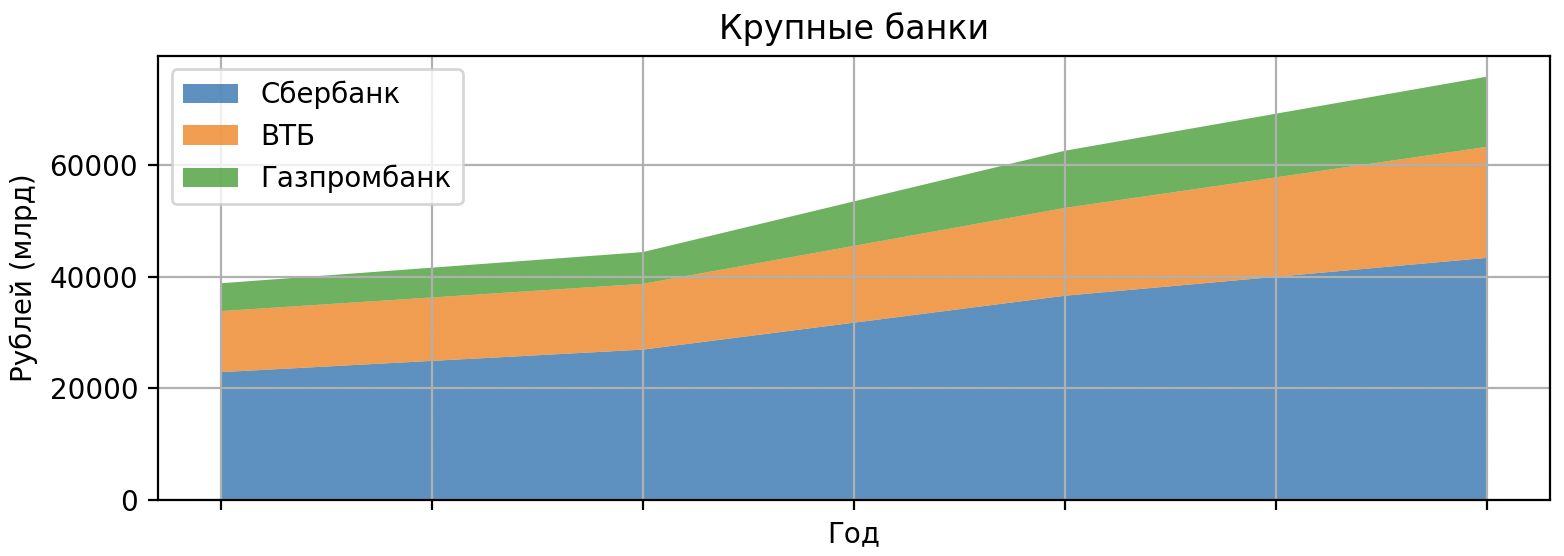
\includegraphics[width=\textwidth]{кредитный_портфель_банков_крупные}
	\caption{Динамика изменений кредитного портфеля крупных банков РФ}
	\label{fig:кредитный_портфель_банков_крупные}
\end{figure}

На Рисунке \ref{fig:кредитный_портфель_банков_малые} представлена динамика
изменений кредитного портфеля банков России, которые находятся в конкуренции с
АКБ <<Абсолют Банк>>.

\begin{figure}[H]
	\centering
	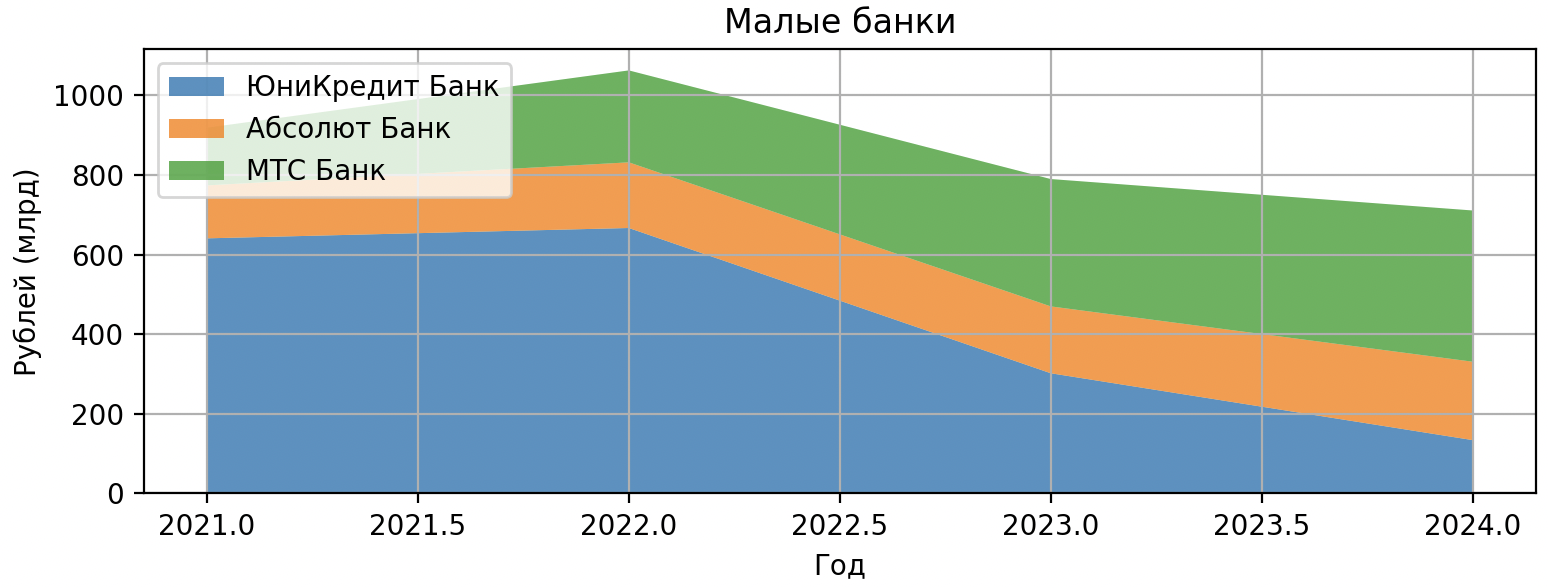
\includegraphics[width=\textwidth]{кредитный_портфель_банков_малые}
	\caption{Динамика изменений кредитного портфеля банков РФ}
	\label{fig:кредитный_портфель_банков_малые}
\end{figure}

Функции модуля потребительского кредитования АКБ <<Абсолют Банк>> типичны для
банковского сектора и включают в себя следующее. Основной функций, которая
охватывает работу с данными является управление данными клиентов. Хранение
такой личной информации клиентов, так имя, адрес, контакты. Хранение данных о
расходах и доходах и кредитной истории. Такие данные применяются для оценки
кредитоспособности и соблюдения требований KYC и AML, что является
необходимостью для предотвращения финансовых преступлений.

Отдельной функцией в потребительском кредитовании является обработку заявок на
кредиты -- это прием и проверка заявок на ипотеку, кредиты и автокредиты,
которая требует верификации документов, оценку кредитного риска и определение
условий кредитования. В условия кредитования входят такие параметры, как сумма,
процентная ставка и срок. Обработка заявок на кредитование включает в себя
процесс запроса дополнительных документов в случае недостатка информации по
тем, которые запрашиваются автоматически для всех кредиторов. Одним из
процессов является применение моделей кредитного скоринга и использование
данных кредитных бюро для анализа кредитоспособности кредитора. В случае с
ипотеками проводится оценка недвижимости для определения ее рыночной стоимости.
<<Абсолют Банк>> позволяет клиентам подавать заявки на кредитование с
использованием онлайн-ресурсов и в отделении банка. На данный момент можно
заметить недостаточно оптимизированные процессы для создания и обработки заявок
с использованием онлайн-портала, так как крупные банки у которых эти процессы
оптимизированы имеют кредитный портфель многократно превышающий портфель банка
<<Абсолют>>.

Одной из основных функцией является выдача кредитов. Процесс выдачи для ипотек
считается завершенным на стадии, где заемщик подписывает документы и получает
ключи от недвижимости, а для других методов кредитования в момент когда
средства переведены на счет заемщика.

Функция обслуживания состоит из перевода средств
заемщику и управления процессом погашения выданных кредитов, что включает в
себя обработку платежей, отслеживание просрочек и работу с дефолтами. Банк
отслеживает своевременность выполнения платежей и отслеживает просроченные
задолженности, в случае просроченных задолженностей банк держит за собой право
инициировать процедуру реструктуризации долга, взыскания или передачи долга в
коллекторское агентство. Это требует эффективных систем для мониторинга и
управления рисками.

Управление рисками -- это процесс, где применяются методы
мониторинга портфелей и финансов кредиторов. Управление рисками подразумевает
проведение стресс-тестов и внедрение мер по их снижению, таких как страхование
и залог. Процесс первичной оценки рисков производится с использованием
скоринговых моделей и мониторинга портфелей, как до выдачи кредита, так и после
выдачи. Рыночные же риски, которые могут быть связаны с изменениями процентных
ставок или валютных курсов решаются с использованием хеджирования и других
финансовых инструментов.

Важнейшим бизнес процессом в банках является генерация отчетности о финансовых
результатах, анализе рисков и производительности различных подразделений,
которые могут применяться менеджментом для принятия стратегических решений.
Финансовые отчеты о балансах, прибылях и убытках предоставляются акционерам и
регуляторам. Отчеты для центрального банка России показывают данные о кредитных
портфелях и соблюдении нормативов.

АКБ <<Абсолют Банк>> обрабатывает такие типы данных, как личная информация,
финансовая история и документы. Данные об объектах кредитования, такие как
адрес, стоимость и отчеты об оценке для ипотек и марка, модель и цену для
автокредитов. Данные о заявках на кредитование, такие как цель, срок,
процентная ставка, графики платежей. Транзакционные данные, которые
подразумевают информацию о платежах, комиссиях и штрафах за просрочку. Рейтинги
рисков, информация о залоге, результаты стресс-тестов кредиторов и регуляторные
данные, которые состоят из отчетов Центральному банку РФ.

\subsection{Предпроектное обследование объекта исследования}

Обследование объекта исследования -- это важный этап, который позволит
собрать, а в результате и визуализировать информацию о текущем состоянии
ИТ-инфраструктуры модуля потребительского кредитования ПАО <<Абсолют Банк>>. В
этом пункте будут рассматриваться модели бизнес-процессов <<как есть>> в
нотации BPMN 2.0, диаграммы UML вариантов использования и DFD, на основе
анализа будут вынесены формальные и неформальные требования к улучшенной
ИТ-инфраструктуре.

На текущий момент бизнес процесс выдачи кредита через веб-приложение включает в
себя четыре актора, а ключевыми являются клиент, менеджер и кредитный
специалист. Эти акторы осуществляют действия по сопровождению, анализу
кредитоспособности, обращению в кредитное бюро и принятию решения по выдаче
кредита. Одним из внешних акторов является аудитор без которого в силу законов
РФ процесс выдачи кредита потребителю не был бы сформирован полностью, так как
для выдачи потребительских кредитов информацию о кредиторах, сроках и ставках
нужно передавать кредитору. На Рисунке\;\ref{fig:uml_use_case} изображена UML
диаграмма вариантов использования бизнес-процесса выдачи кредита.

\begin{figure}[H]
	\centering
	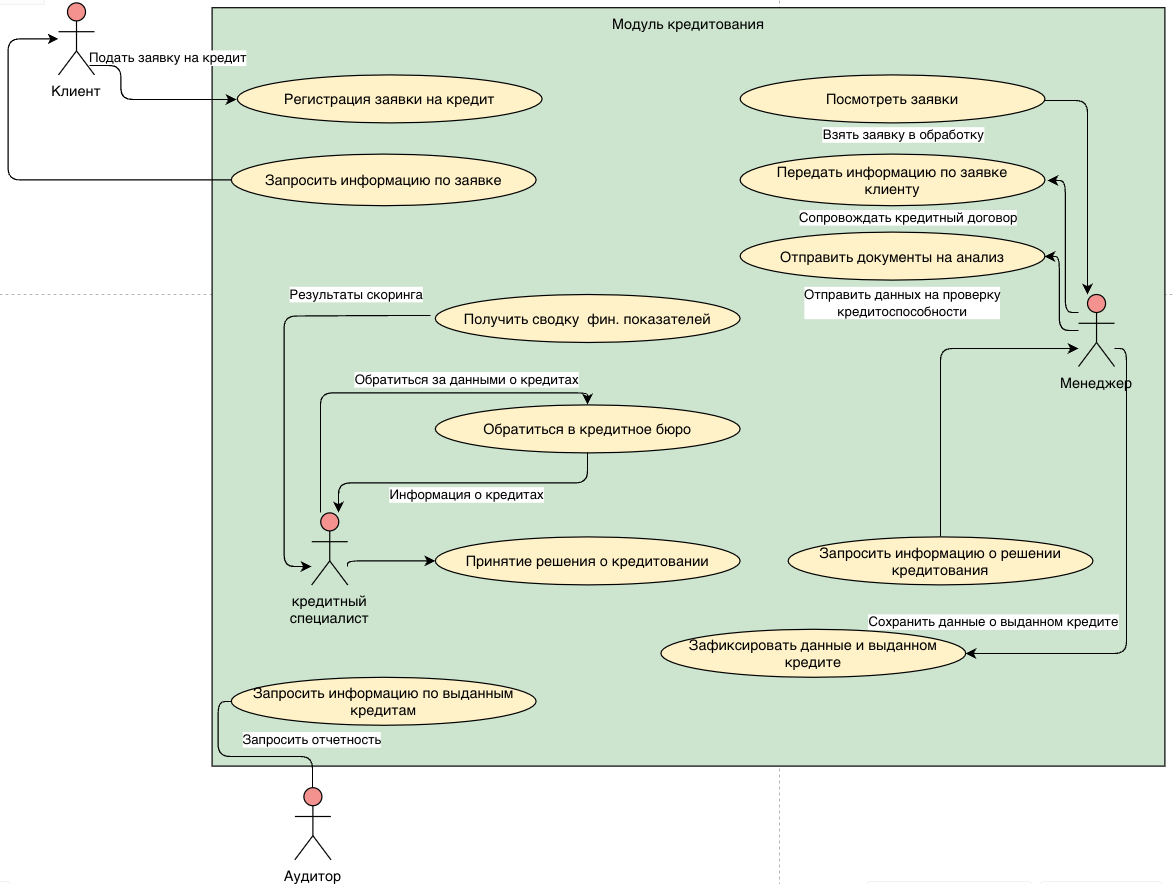
\includegraphics[scale=0.38]{uml_use_case_extended}
	\caption{Диаграмма UML вариантов использования процесса кредитования}
	\label{fig:uml_use_case}
\end{figure}

Текстовое описание UML диаграммы вариантов использования представлена в Таблице
\ref{tab:table_use_case}. В диаграмме используются только связи обобщения.

\begin{tabularx}{\textwidth}{|l|X|X|}
	\captionsetup{margin=-14pt}
	\caption{Текстовое описание вариантов использования\label{tab:table_use_case}}
		\\
	\endfirsthead
	\caption*{Продолжение таблицы~\ref{tab:table_use_case}} \\
	\hline
	№ & Актор 		       	  & Действие 					 				  \\\hline
	\endhead
	\endfoot
	\endlastfoot

	\hline
	№  & Актор 				  & Действие 					 				  \\\hline
	1  & Клиент 			  & Регистрация заявки на кредит  				  \\\hline
	2  & Клиент 			  & Запросить информацию по заявке 				  \\\hline
	3  & Менеджер 			  & Посмотреть заявки на кредит   				  \\\hline
	4  & Менеджер 			  & Передать информацию по заявке клиенту   	  \\\hline
	5  & Менеджер 			  & Отправить документы на анализ   			  \\
	6  & Менеджер 			  & Запросить информацию о решении кредитования   \\\hline
	7  & Менеджер 			  & Зафиксировать данные о выданном кредите   	  \\\hline
	8  & Кредитный специалист & Получить сводку финансовых показателей
клиента\\\hline
	9  & Кредитный специалист & Обратиться в кредитное бюро 				  \\\hline
	10 & Кредитный специалист & Принять решение о кредитовании 			 	  \\\hline
	11 & Аудитор 	 		  & Запросить информацию по выданным кредитам 	  \\\hline
\end{tabularx}
Проанализировав диаграмму вариантов использования можно понять, что
бизнес-процесс выдачи кредитов с использованием веб-приложения находится на
высоком уровне цифровизации, но стоит обратить внимание на большое количество
действий, которые выполняются кредитным специалистом. Из действий выполняемых
кредитным специалистом можно избавиться от обращения в кредитное бюро
автоматизацией и вынесением этого в интеграцию с собственной CRM системой. Так
же можно избавиться от действия фиксации данных о выданном кредите, которое
выполняется актором <<менеджер>>, так как данные можно фиксировать в процессе
передачи между акторами.

На Рисунке \ref{fig:dfd0} представлена контекстная диаграмма
процесса создания заявки на кредитование клиентом через интерфейс
веб-приложения с применением нотации DFD (диаграмма потоков данных). На
Рисунке \ref{fig:dfd1} представлена декомпозиция контекстной диаграммы. На
декомпозированной диаграмме показаны основные потоки данных поступающих от
клиента, используемых внутри модуля и так же их передача за рамки модуля в
кредитное бюро для получения истории кредитов клиента, что необходимо для
точного определения кредитоспособности. Можно увидеть, что за каждым новым
запросом клиента нужно передать заявки в систему скоринга, что можно
оптимизировать сохранением результатов скоринга и в будущем при повторном
обращении через небольшое время вместо проведения повторного скоринга
воспользоваться результатами уже проведенного скоринга.

\begin{figure}[H]
	\centering
	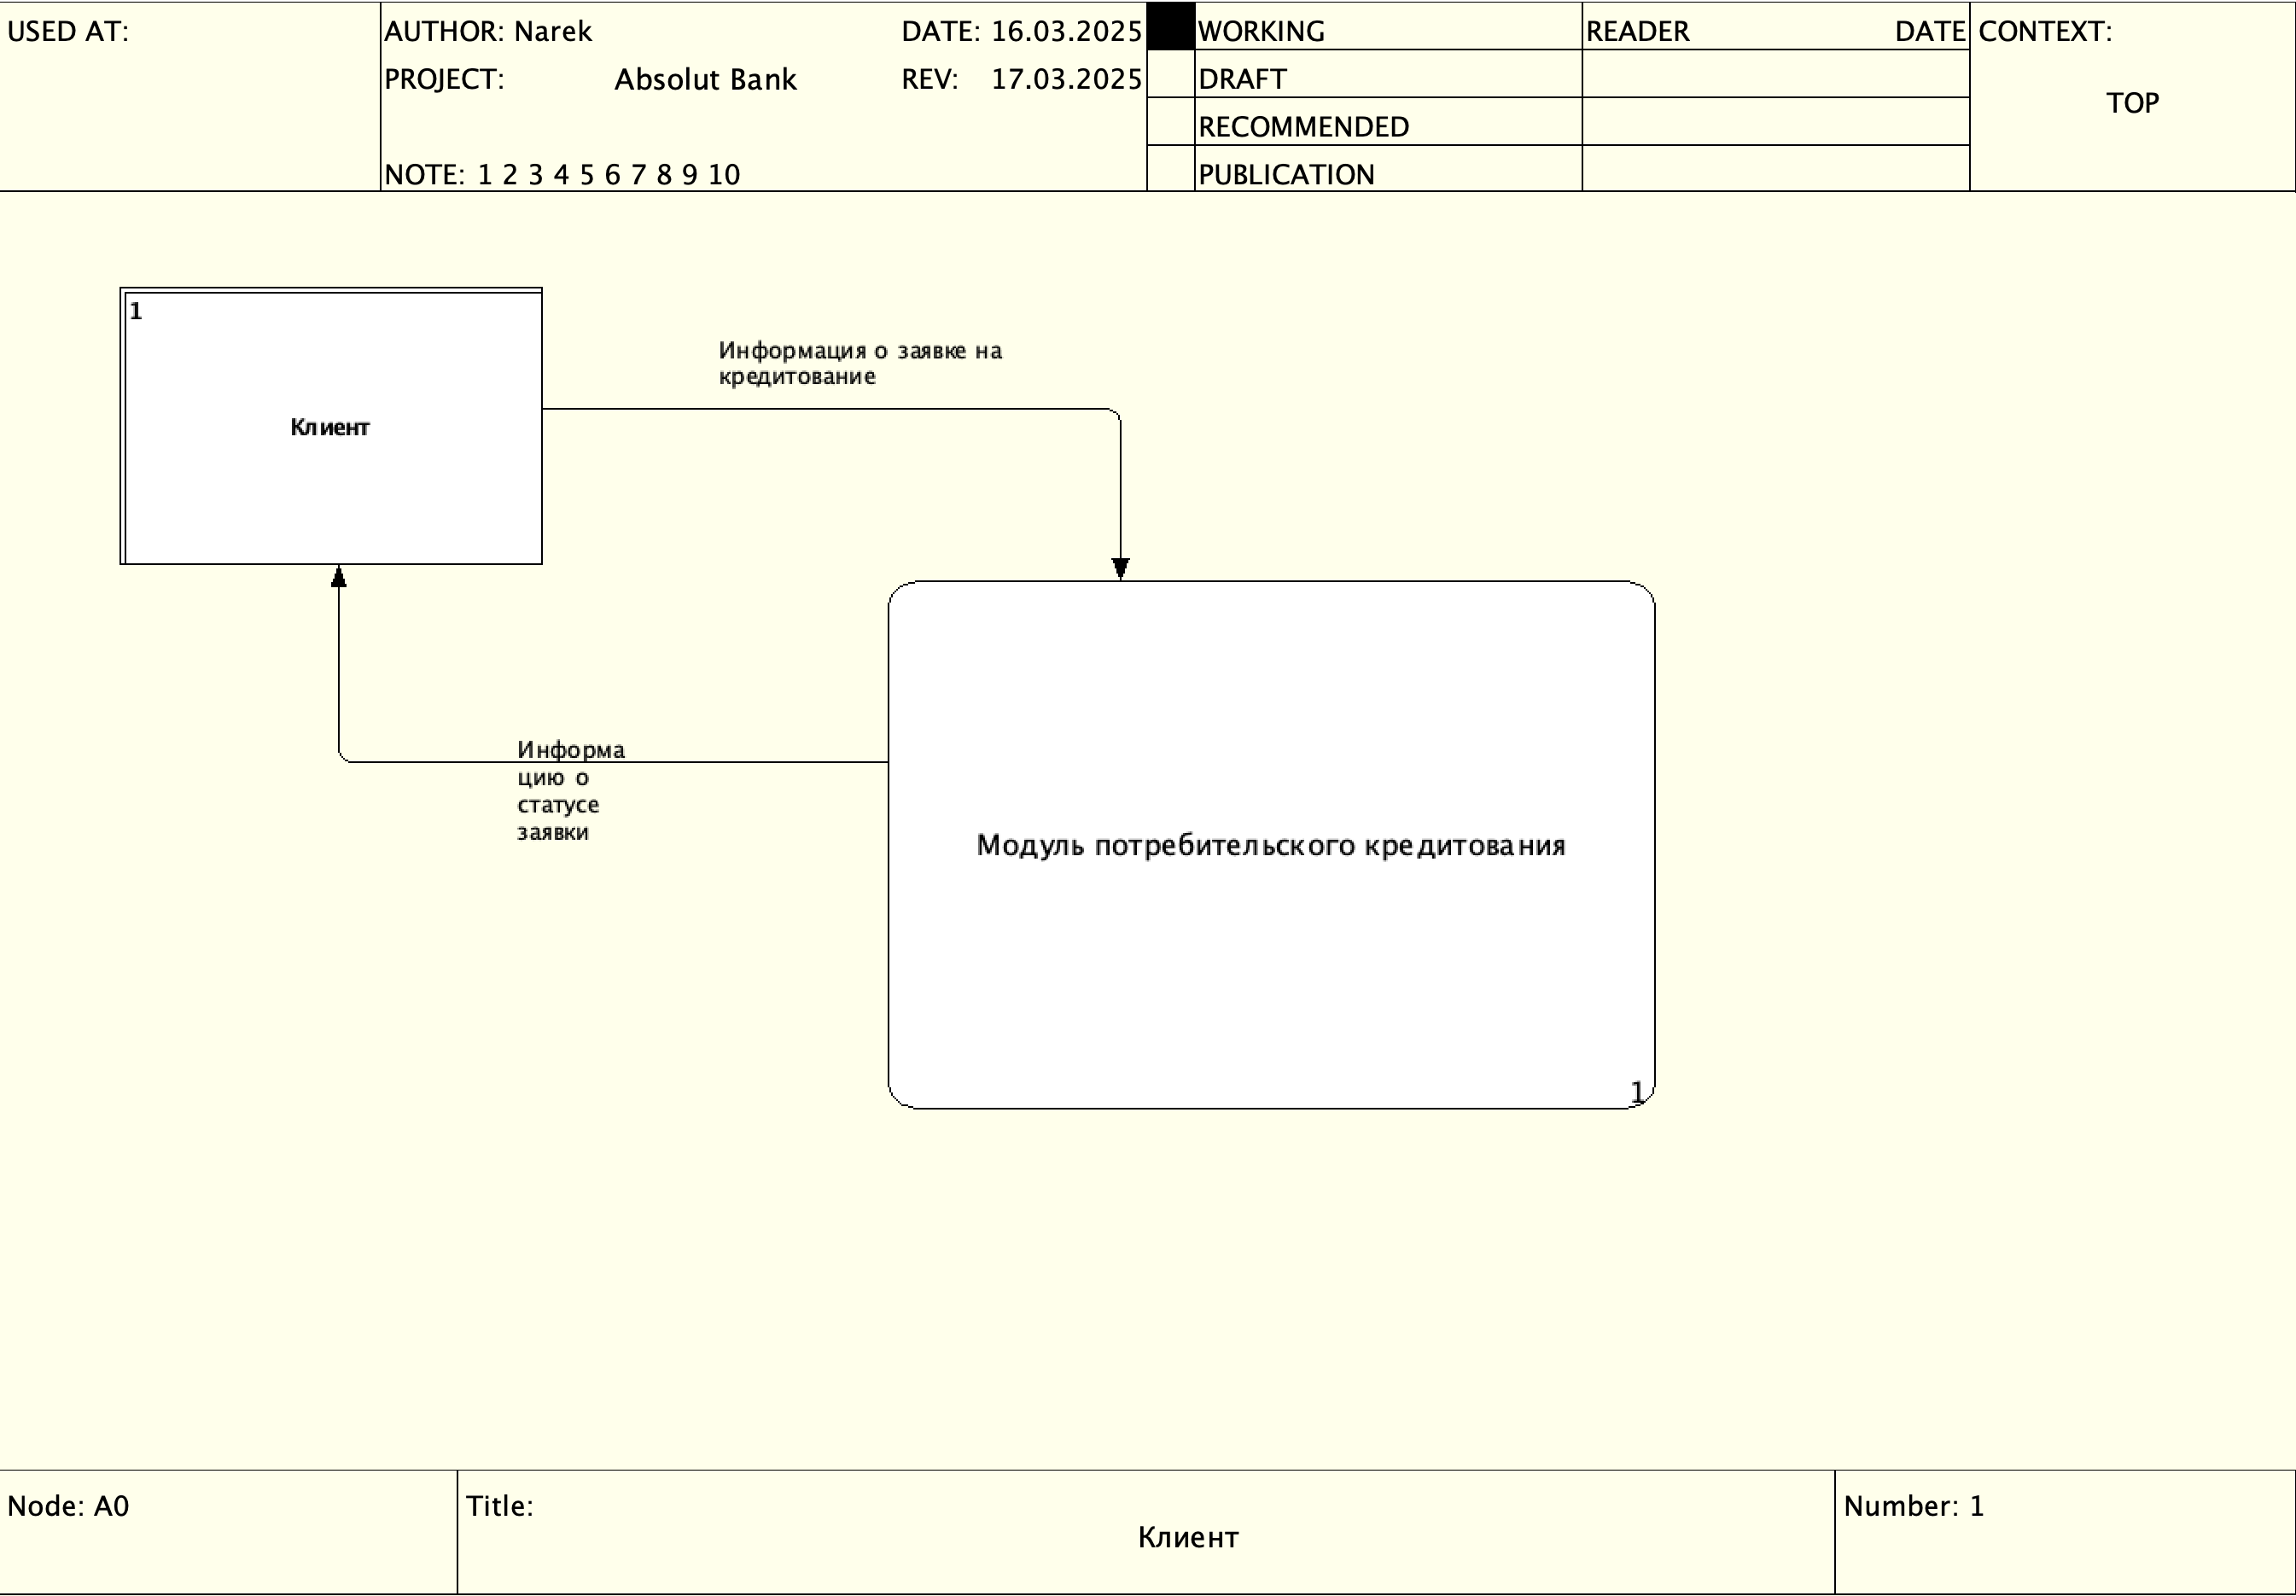
\includegraphics[scale=0.33]{dfd0}
	\caption{Контекстная диаграмма DFD процесса создания заявки на кредитование}
	\label{fig:dfd0}
\end{figure}

\begin{figure}[H]
	\centering
	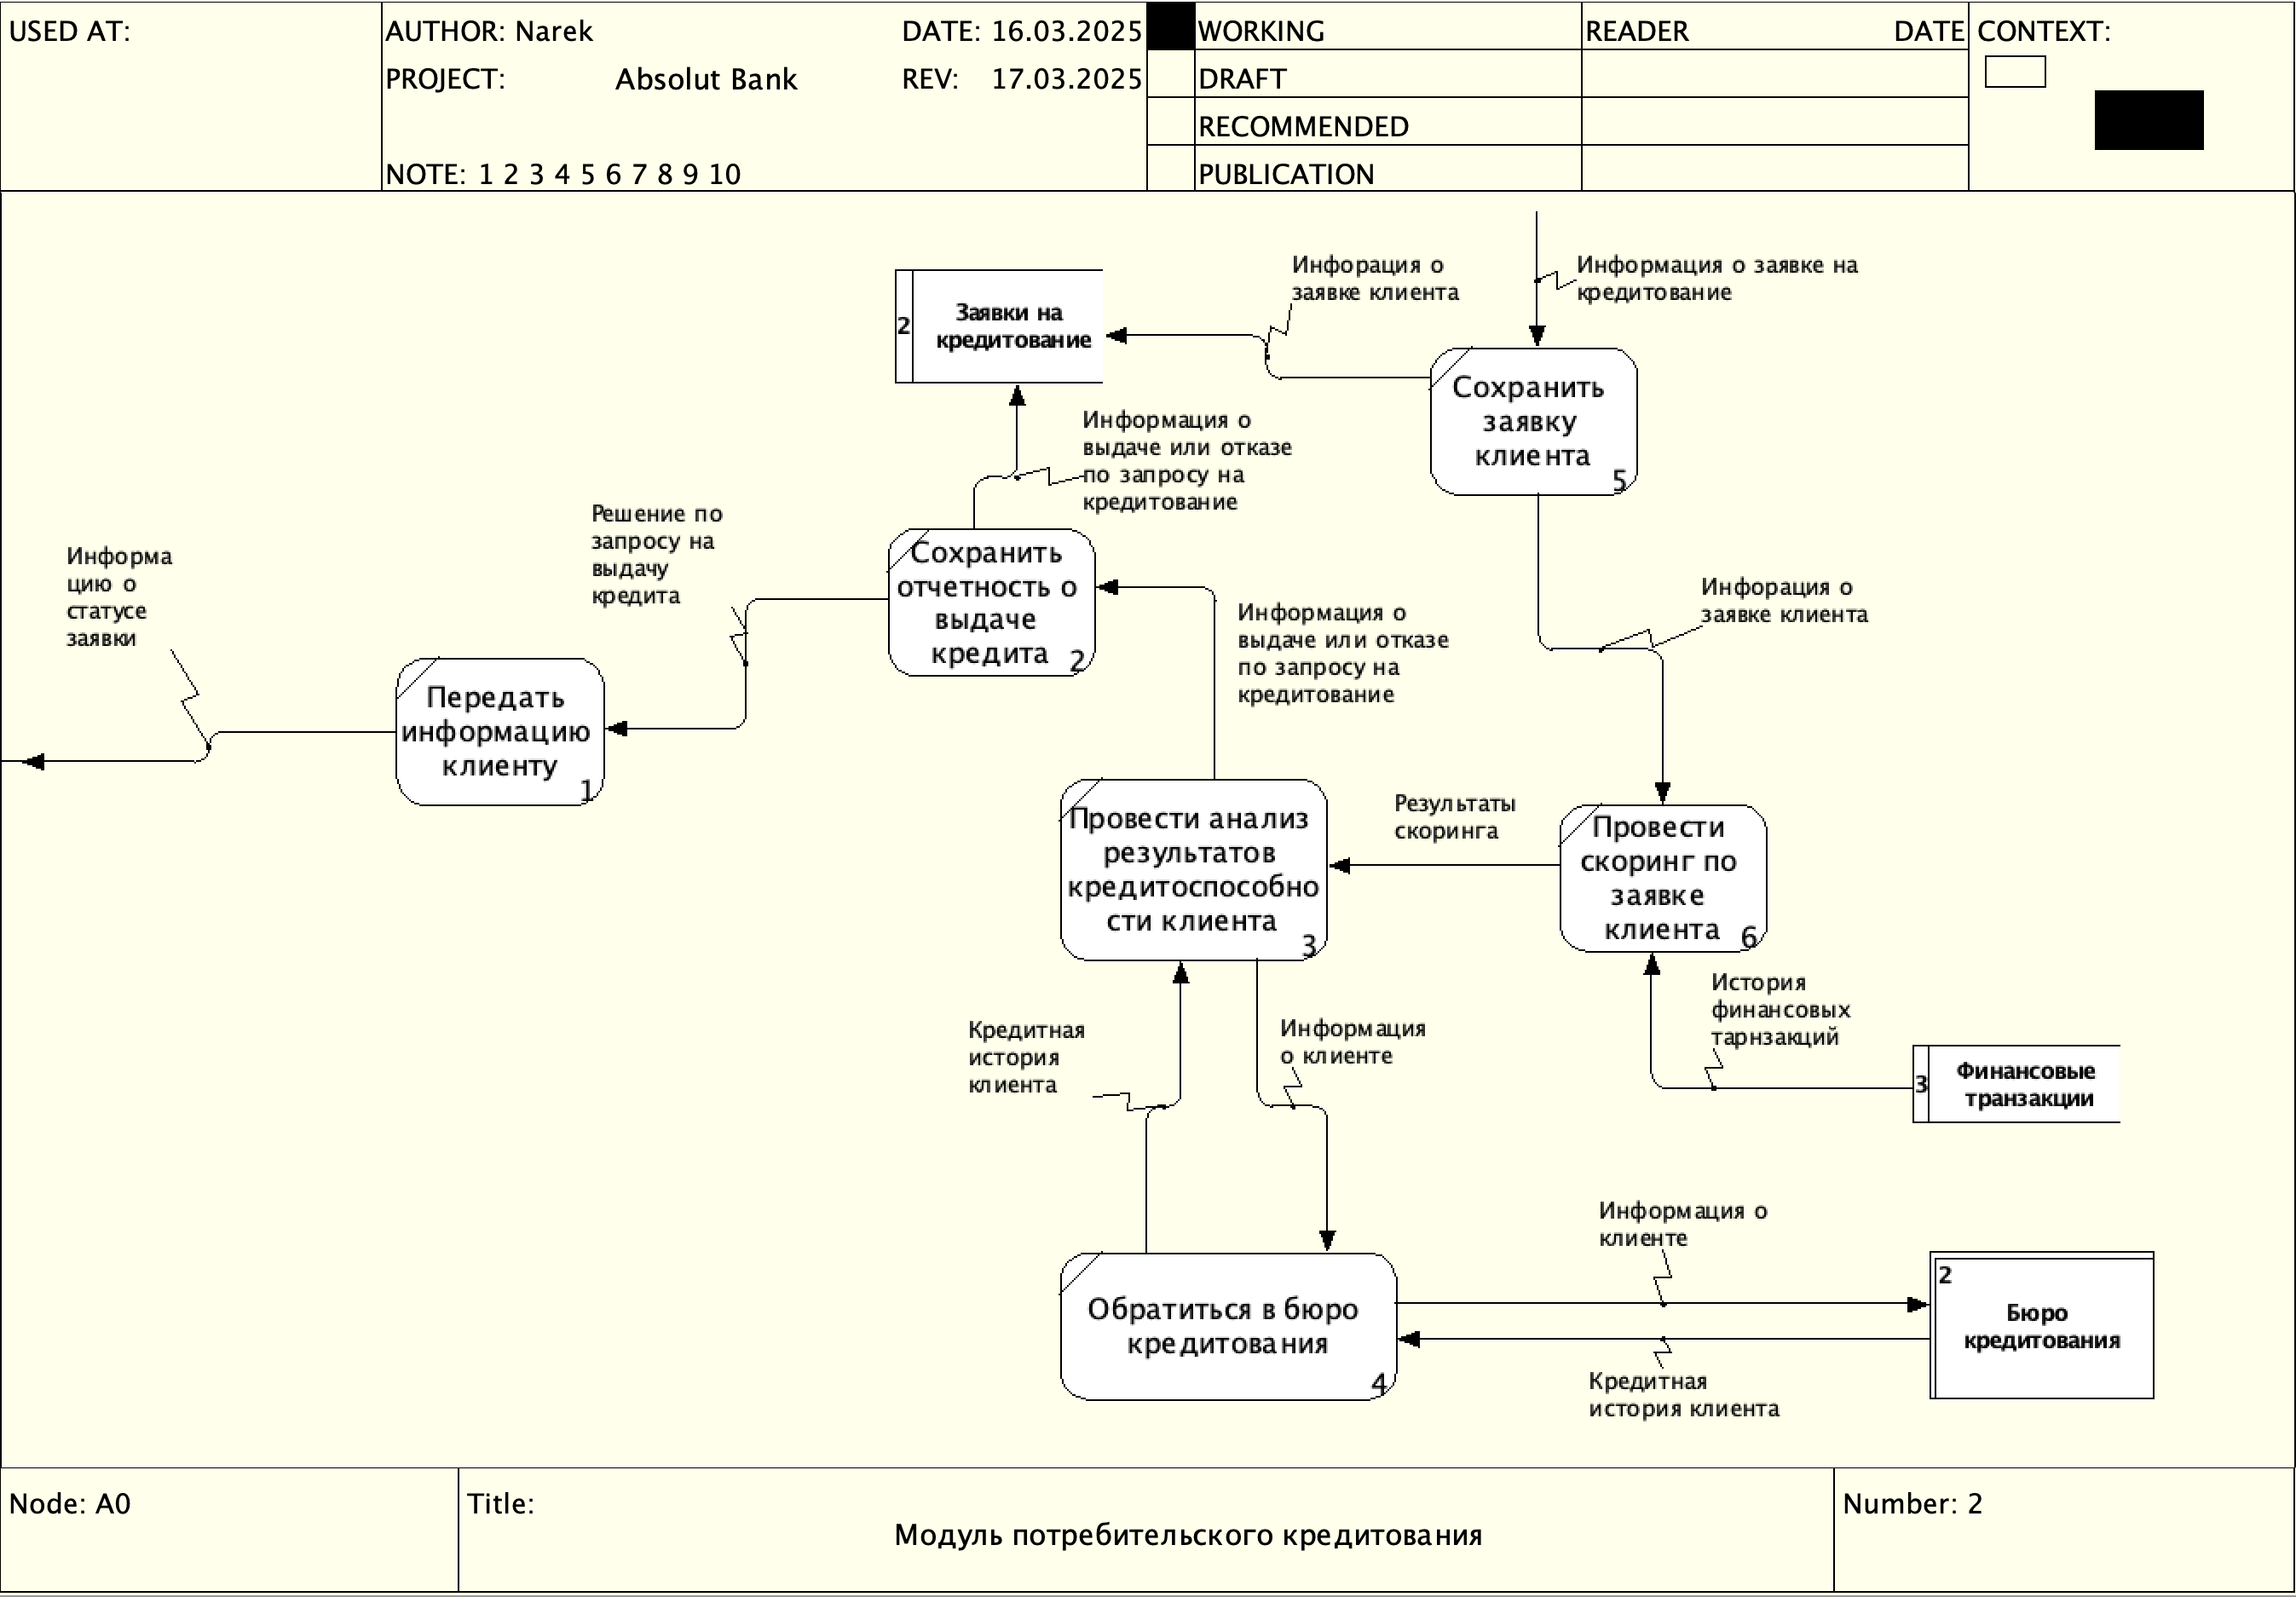
\includegraphics[scale=0.33]{dfd1}
	\caption{Декомпозиция контекстной диаграммы DFD процесса создания заявки на
кредитование}
	\label{fig:dfd1}
\end{figure}

Компоненты ИТ-инфраструктуры и технологии, которые в фокусе модуля
потребительского кредитования АКБ <<Абсолют Банк>> включают в себя системы баз
данных, системы и средства обеспечения безопасности, функциональные модули,
интеграции и пользовательский интерфейс. На Рисунках \ref{fig:bpmn0} -
\ref{fig:bpmn1} представлены технологии и процессы происходящие в рамках
оформления потребительского кредиты.

\begin{figure}[H]
	\centering
	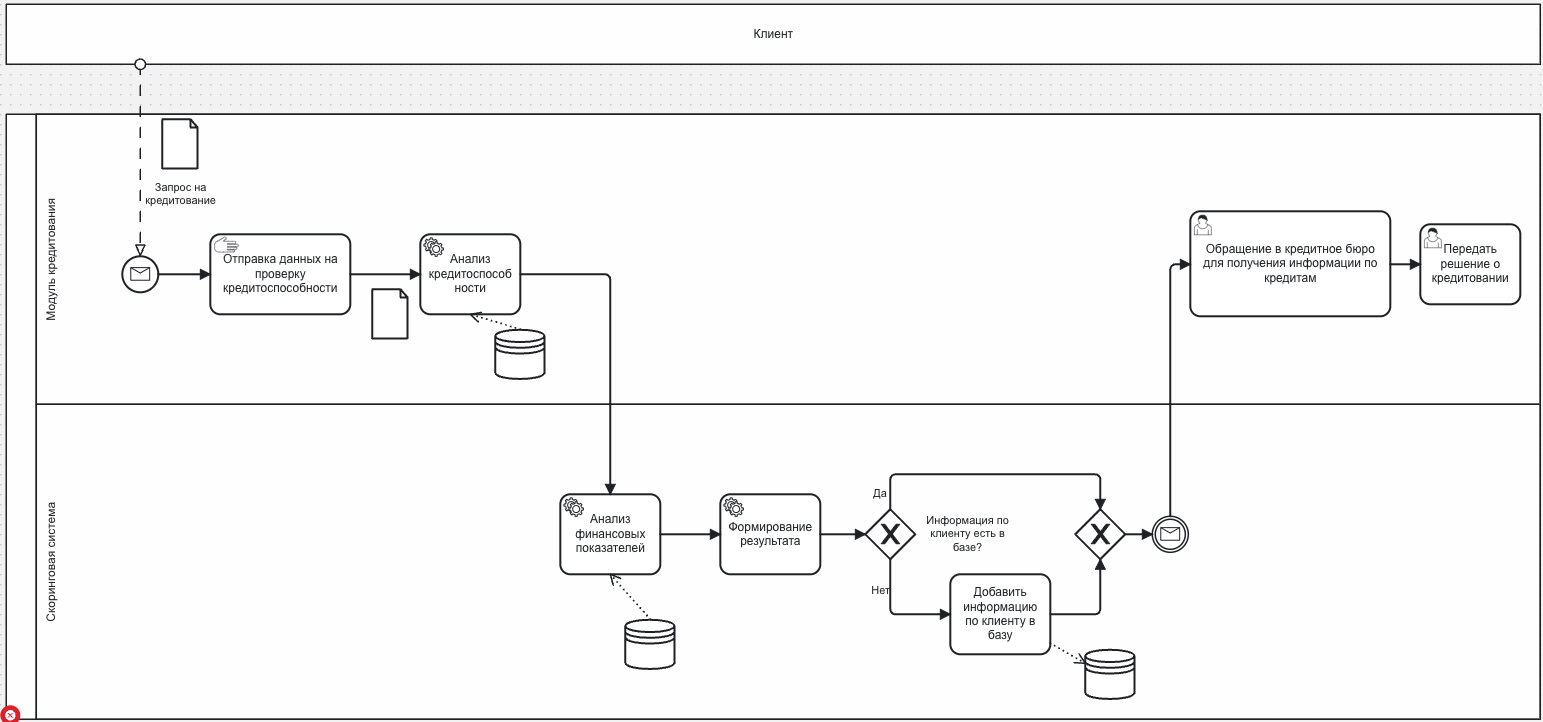
\includegraphics[scale=0.3]{bpmn_diagram_0.png}
	\caption{Диаграмма BPMN бизнес-процессов}
	\label{fig:bpmn0}
\end{figure}

\begin{figure}[H]
	\centering
	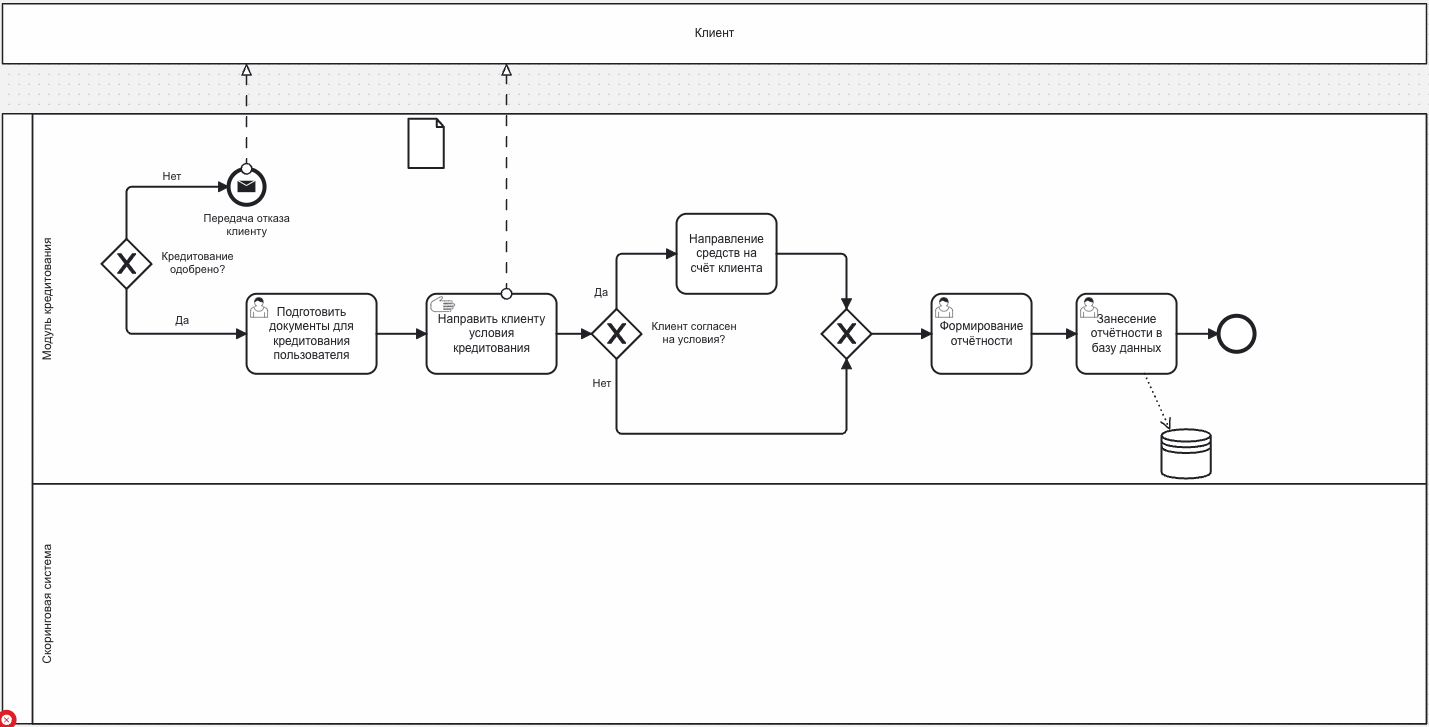
\includegraphics[scale=0.33]{bpmn_diagram_1.png}
	\caption*{Продолжение рисунка \ref{fig:bpmn0}}
	\label{fig:bpmn1}
\end{figure}

АКБ <<Абсолют банк>> для хранения данных использует SQL хранилище данных,
такое как <<Oracle Database>>, и NoSQL хранилище <<MongoDB>>. Для мониторинга
компания используется и сбора метрик модуль использует программное обеспечение
<<Yandex metrica>>\;\cite{absolut-infrastructure-usage}. Основным инструментом
для бизнес-аналитики в компании является ПО <<Power BI>>. Системы управления
кредитами, так как скоринговая  система, система верификации, система расчета
кредитного лимита у компании свои, то есть в правлении кредитами компания не
пользуется готовыми решениями. Инструменты для управления рисками у компании
так же свои, готовые решения в этом блоке компания не использует. CRM система
и весь остальной комплекс инструментов для автоматизации части
бизнес процессов, маркетинговых коммуникаций и обработки лидов
продаж используется <<BPMSoft>>\;\cite{BPMSoft-usage}. Для обеспечения
безопасности инфраструктуры используется ПО от производителя Positive
Tecnologies <<MaxPatrol>>\;\cite{absolut-MaxPatrol-usage}. Так как в банковском
секторе требуется возможность иметь интеграцию с больших количеством
сервисов и получать информацию от них, для этого нужен мощный инструмент
обеспечивающий скорость интеграции, для этого используется ПО <<BidSwitch>>. В
Таблице \ref{tab:infra-coast} показано все аппаратные ресурсы арендуемые на
<<Google cloud>>, их количество и стоимость. Общая стоимость всех облачных
аппаратных ресурсов и обслуживаемых ресурсов составляет 3.290.000 рублей каждый
месяц и 39.480.000 в год.

\begin{tabularx}{\textwidth}{|l|X|X|X|X|}
    \captionsetup{margin=-14pt}
    \caption{Стоимость и количество арендуемого ПО.\label{tab:infra-coast}}
    \\
	\endfirsthead
	\caption*{Продолжение таблицы~\ref{tab:infra-coast}} \\
	\hline
    № & Компонент                & Характеристики                        &
Количество & Стоимость единицы в месяц \\ \hline
	\endhead
	\endfoot
	\endlastfoot

    \hline
    № & Компонент                & Характеристики                        &
Количество & Стоимость единицы в месяц \\ \hline
	1 & Виртуальная машина       & Ubuntu 24.4, 8v CPU, 16G RAM, 3TB SSD & 4     

	& 70.000 рублей             \\ \hline
	2 & Обслуживаемый PostgreSQL & 24v CPU, 96GB RAM                     & 2     

	& 300.000 рублей            \\ \hline
	3 & Обслуживаемый MongoDB    & 24v CPU, 96GB RAM                     & 1     

	& 130.000 рублей            \\ \hline
	4 & Хранилище                & 86 TB SSD, 40 000 IOPS                & 2     

	& 1.140.000 рублей          \\ \hline
\end{tabularx} 

АРМ офиса клиентской поддержки блока кредитования представляют из
себя компьютеры средней мощности достаточной для обработки заявок, которые
подаются клиентами в офисе. Характеристики АРМ представлены в Таблице
\ref{tab:arm_hardware}. Стоимость одного АРМ с характеристиками представленными
ниже составляет примерно 40 000 рублей.

\begin{tabularx}{\textwidth}{|l|X|X|X|}
    \captionsetup{margin=-14pt}
    \caption{Текстовое описание вариантов
использования\label{tab:arm_hardware}}
    \\
	\endfirsthead
	\caption*{Продолжение таблицы~\ref{tab:arm_hardware}} \\
	\hline
	№  & Компонент  & Модель              & Характеристики \\\hline
	\endhead
	\endfoot
	\endlastfoot

    \hline
    №  & Компонент  & Модель              & Характеристики \\\hline
    1  & Процессор  & Intel Core i3-4130  & Двухъядерный, 4 потока, базовая
частота 3,40 ГГц, кэш 3 МБ, встроенная графика Intel HD Graphics 4400
\cite{intel-corei3-4130}. \\\hline
    2  & ОЗУ        & DDR4 8 ГБ 2400 МГц  & Тип DDR4 SDRAM, частота 2400 МГц,
форм-фактор DIMM, напряжение питания 1,2 В. \\\hline
    3  & Хранилище  & SSD SATA III 512 ГБ & Скорость чтения до 560 МБ/с,
скорость записи до 535 МБ/с, интерфейс SATA III. \\\hline
    4  & Интернет   & Ethernet 100 Мбит/с & Надежное подключение к сети,
достаточное для большинства офисных задач. \\\hline
    5  & Видеокарта & Intel UHD Graphics  & Встроенная графика, достаточная для
офисных приложений. \\\hline
\end{tabularx}

Работникам компании, которые работают в удаленном формате или рабочим местом не
является прикрепленное за ними окно для обработки заявок клиентов, выдаются
ноутбуки <<Aquarius AQbook NE355>> \cite{aquarius-aqbook-NE355} для
мобильности. Стоимость одного ноутбука <<Aquarius AQbook NE355>> составляет 88
000 рублей для не коммерческого потребителя, но в связи с тем, что компания
выпускает свои ноутбуки именно для коммерческого пользования, то цены в таком
случае ниже.

В Таблице \ref{tab:soft-coast} представлено программное используемое на АРМ
сотрудников и их стоимость.

\begin{tabularx}{\textwidth}{|l|X|X|}
    \captionsetup{margin=-14pt}
    \caption{ПО для АРМ сотрудников и его стоимость\label{tab:soft-coast}}
    \\
	\endfirsthead
	\caption*{Продолжение таблицы~\ref{tab:soft-coast}} \\
	\hline
	№ & Программное обеспечение & Стоимость единицы в месяц \\ \hline
	\endhead
	\endfoot
	\endlastfoot

    \hline
	№ & Программное обеспечение & Стоимость единицы в месяц \\ \hline
	1 & Micrasoft office        & 1200 рублей               \\ \hline
	2 & Micrasoft windows 11    & 1100 рублей               \\ \hline
\end{tabularx} 

При столь внушительных объемах обрабатываемых данных, строгом регулировании
сектора банкинга и кредитования в РФ и количестве интеграций можно понять, что
облачное решение для компании уже не является выгодным и безопасным. К тому же
облачные вендоры не всегда гарантируют, что данные, которые хранятся на их
устройствах будут в полной сохранности и никогда не будут утеряны, а это
ключевой фактор для отрасли деятельности АКБ <<Абсолют Банк>>.

\subsection{Характеристика предмета исследования}

В этом пункте сформирована совокупность целевых уровней качества обслуживания,
системных требований к программному обеспечению и процессу хранения и обработки
данных. Этот пункт формирует понимание о том на каком уровне на данный момент
обеспечивается качество и скорость обслуживания клиентов, хранятся
чувствительные данные о клиентах и их финансовая информация, насколько быстро и
качественно работают такие системы для функционирования кредитования, как
скоринговая система и система рискового анализа. В этом пункте описано как
справляется нынешняя инфраструктура с существующими нагрузками, то как часто
происходят происшествия связанные с инфраструктурой и то сколько времени
требуется на устранение. Данные об уровне обслуживания клиентов существующие на
данный момент позволят понять какие есть слабые места в обслуживании, что
укажет на недостатки в системе хранения и обработки данных.

Для определения системных требований к ИТ-инфраструктуре требуется определить
все продуктовые показатели которыми на данный момент обладает система. К
показателям потребительского кредитования можно отнести: 
\begin{enumerate}
	\item Скорость оформления кредита.
	\item Время рассмотрения заявки.
	\item Количество предлагаем видов кредитования.
	\item Риск утери данных.
	\item Количество документов требуемых от клиента.
\end{enumerate}

Результаты продуктовых SLA, которые показывает на данный момент модуль
потребительского кредитования АКБ <<Абсолют Банк>> представлены в Таблице
\ref{tab:SLA-business}.

\begin{tabularx}{\textwidth}{|l|X|X|}
    \captionsetup{margin=-14pt}
    \caption{Бизнес показатели качества обслуживания\label{tab:SLA-business}}
    \\
	\endfirsthead
	\caption*{Продолжение таблицы \ref{tab:arm_hardware}} \\
	\hline
    №  & Показатель & Значение \\\hline
	\endhead 
	\endfoot
	\endlastfoot

    \hline
    №  & Показатель & Значение \\\hline
    1  & Скорость оформления заявки & 30 минут \\\hline
    2  & Время рассмотрения заявки & 2-3 рабочих дня \\\hline
    3  & Количество предлагаем видов кредитования в веб-приложении & 1,
потребительский
\\\hline
    3  & Количество предлагаем видов кредитования в офисе & 3, потребительский,
автокредит, ипотека \\\hline
    4  & Риск утери данных & Низкий-средный (данные хранятся в облаках)
\\\hline
    5  & Количество документов требуемых от клиента & 2-5 (паспорт, СНИЛС,
подтверждение дохода) \\\hline
    6  & Уровень удовлетворенности & Высокий (оценка 4 на основе отзывов
клиентов) \\\hline
    7  & Процент одобрения заявок & 70-80\% \\\hline
    8  & Средний размер кредита & 600 000 рублей \\\hline
    9  & Процентная ставка по кредитам & 12-18\% годовых \\\hline
    10 & Количество активных клиентов & 50 000 - 60 000 \\\hline
\end{tabularx}

В Таблице \ref{tab:SLA-tech} отображены основные технические показатели
выдаваемые ИТ-инфраструктурой модуля потребительского кредитования АКБ
<<Абсолют Банк>>.

\begin{tabularx}{\textwidth}{|l|X|X|}
	\captionsetup{margin=-14pt}
	\caption{Технические показатели и ИТ-инфраструктура\label{tab:SLA-tech}}
	\\
	\endfirsthead
	\caption*{Технические показатели и ИТ-инфраструктура\ref{tab:SLA-tech}} \\
	\hline
	№  & Показатель & Значение \\\hline
	\endhead
	\endfoot
	\endlastfoot
	\hline
	№ & Показатель & Значение \\\hline
	1 & Тип хранения данных & Облачное хранение (Google Cloud) \\\hline
	2 & Объём хранилища данных & 176 ТБ \\\hline
	3 & Базы данных & Oracle, MongoDB \\\hline
	4 & Уровень защиты данных & Средний-высокий (резервные копии) \\\hline
	5 & Скорость обработки данных & 600 транзакций в секунду \\\hline
	6 & Время восстановления данных после сбоя & 4 часа \\\hline
	7 & Время реагирования на инциденты & 20 минут \\\hline
	8 & Уровень доступности системы & 99.89\% \\\hline
	10 & Количество облачных серверов & 4 сервера \\\hline
	11 & Используемые протоколы безопасности & HTTPS, SSL/TLS \\\hline
\end{tabularx}

По результатам рассмотрения продуктовых и технических показателей существующей
системы можно придти к выводу, что уровень доступности у банка довольно низок,
а большинство компаний в сфере банкинга придерживаются значения 99,99\%, так
же
стоит
обратить
внимание на показатель уровня защиты данных. Уровнь защиты данных в первую
очередь должен соответствовать всем мировым стандартам и законам РФ, кроме того
базы данных должны иметь резервную копию в нескольких экземплярах. Банк всегда
должен иметь копию базы соответствующую данным на данный момент с отклонением
до одной секунды. Для банковской системы хранение данных в облачной
инфраструктуре является отрицательным показателем, так как гарантии вендора
могут не оправдаться, а потеря данных не допустима.

Среднее время обработки заявок напрямую коррелируется с тем как устроены
хранение и обработка данных, так как менеджеры и кредитные специалисты
присутствуют в достаточном количестве, что снижает вероятность задержек по
человеческому фактору. Это значит, что время ожидания данных из базы данных и
ответа скоринговой системы велики. Скоринговая система полностью построена на
анализе транзакционной информации клиента и причиной задержек в ее ответе может
являться неверно выбранная или перегруженная база данных. В среднем время
обработки заявки на потребительское кредитование для 90\% заявок составляет 72
часа, что превышает среднее время обработки в других банках. Этот результат
можно улучшить сохраняя и корректно используя данные клиентов, которые уже
зарегистрированы в банковской системе.

АКБ <<Абсолют Банк>> использует современные технологии для мониторинга и
логирования произшествий, что отражается в небольшом времени реагирования, но
время устранения ошибок велико в связи с плохим описание ИТ-инфраструктуры и
плохим выбором вендора облачной инфраструктуры, так как пользователи Google
Cloud часто сталкиваются со сбоями в работе веб-сайта, а это может
сыграть ключевую роль в момент инцидента (Рисунок
\ref{fig:google_cloud_downtime}).

\begin{figure}[H]
	\centering
	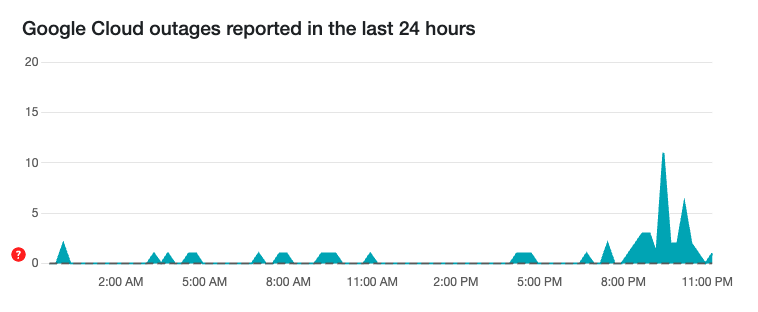
\includegraphics[scale=0.48]{google_cloud_downtime.png}
	\caption{Сообщения о сбоях в облаке Google 17 марта 2025 года}
	\label{fig:google_cloud_downtime}
\end{figure}

\subsection{Архитектура объекта исследования}

Архитектура объекта исследования -- это текущая (<<как-есть>>) модель
ИТ-инфраструктуры, которая поддерживает модуль потребительского кредитования
АКБ <<Абсолют Банк>>. Архитектура состоит из трех слоев: бизнес-слой, слой
приложений и технологический слой. На основе доступных данных и типичных
практик в секторе потребительского кредитования в этом пункте описана
архитектура объекта. Для визуализации взаимодействий между всеми слоями
архитектуры используется язык моделирования ArchiMate \cite{archimate-landing}.
Этот модуль дает полноценное понимание о всех бизнес, продуктовых и технических
процессах, которые играют ключевую роль в цепочке действий получения
потребительского кредита в АБК <<Абсолют Банк>>.


Бизнес-слой показывает ключевые процессы, необходимые для предоставления услуг
потребительского кредитования. К процессам бизнес слоя можно отнести процесс
регистрации клиентов, который подразумевает сбор личной информации и финансовой
информации о клиенте. Этот процесс поддерживается CRM системой и системой
хранения данных. Другим важным процессом является обработка заявок на
кредитование в рамках которого производятся прием заявок и дополнительных
данных в случае ипотечного или автокредитования и верификация документов
потребителя. Обработка заявок на кредитование поддерживается системой
управления обучением. Следующим важным бизнес-процессом является утверждение
кредитов, он включает оценку кредитоспособности заявителей, анализ их кредитной
истории и платежеспособности с использованием банковской скоринговой системы.
После утверждения потребительского кредита запускается процесс выдачи
кредита, который описывается перемещением средств на банковский счет
потребителя. Далее запускаются три процесса, которые частично параллельны --
это обслуживание выданных кредитов, управление рисками и отчетность. Каждый из
этих процессов помогает банковской системе обезопасить себя и оптимизировать
взаимодействие контрагентов с системой кредитования, так как обслуживая кредит 
банковская система собирает отчетность по платежам и по их результатам
рассчитывает риски кредитования потребителя.

Слой приложений находится уровнем выше и он поддерживает работоспособность
бизнес слоя предоставляя инструменты и методы взаимодействия с технологическим 
слоем.

Система взаимодействия с клиентами (CRM) -- это основной инструмент для
менеджера и других участников блока благодаря которым они могут удобно
взаимодействовать с клиентами, сохранять информацию о них и так же доносить эту
информацию до клиента в случае каких-либо изменений. Так же благодаря этому
становится возможен процесс регистрации клиентов. Система управления кредитами
обрабатывает весь жизненный цикл кредита, который начинается в момент подачи
заявки и оканчивается погашением. На протяжении жизненного цикла кредита
система риски и уведомляет об этом менеджеров. Инструмент отчетности и
аналитики предназначен в первую очередь для сбора метрик, их анализа и удобного
представления для менеджеров, которые смогут на основе собранных данных
корректировать работу модуля под потребности и желания клиентов, кроме того эта
система является неотъемлемой частью кредитной организации, так как вся
информация собранная в отчеты должна предоставляться государственным органам
управления финансами и активами, например ЦБ России. Роль замой наиболее важной
системы в банковском секторе занимает система безопасности, так как атаки,
взломы и потеря личной информации могут лишить банк лицензии.

Технологический слой ИТ-инфраструктуры является критически важным для
обеспечения надежности, безопасности и масштабируемости системы.

Технологический слой состоит из серверов на которых находится все ПО
обеспечивающее работу веб-сайта, пользовательского приложения. На сервере
развернуты такие системы, как CRM, система управления кредитами, банковская
система, инструменты аналитики и обеспечения безопасности взаимодействия
потребителей с интерфейсами.

Базы данных играет ключевую роль в хранении и управлении данными и она же
является наиболее желаемым со стороны злоумышленников, так как личные данные
пользователей должны храниться в полной недоступности для других участников
системы. База данных должна иметь несколько уровней шифрования и для передачи
данных должны иметь несколько уровней шифрования. По законам РФ не все личные
данные можно хранить в базе не имея лицензий, которые выдаются после проверок
сохранности и данных. База данных должны иметь собственную систему мониторинга
и шифрования, доступ к которым ограничен узким кругом разработчиков.

Технологический слой состоит из серверов, которые в физичеком виде
недоступны, так как они представлены как виртуальные машины для потребителя в
облачной платформе, на которых находится все ПО обеспечивающее работу
веб-сайта, пользовательского приложения. На сервере развернуты такие системы,
как CRM, система управления кредитами, банковская система, инструменты
аналитики и обеспечения безопасности взаимодействия потребителей с
интерфейсами.

Базы данных играет ключевую роль в хранении и управлении данными и она же
является наиболее желаемым со стороны злоумышленников, так как получив до
ступ к личным данным пользователей злоумышленники получаются возможность на
финансовые операции от лица потребителей. Базы данных так же предоставляются
облачным вендором, что добавляет в цепочку звену полностью не подконтрольное
модулю потребительского кредитования, что может вызвать проблемы в случае
ужесточения законов о хранении личных данных пользователей.

Сетевая инфраструктура в офисах АКБ <<Абсолют банк>> довольно проста в
исполнении, так как нет необходимости передавать данные из центра обработки
данных или перемещать их в рамках центра. Для получения доступа к
данных, пользовательским и потребительским ресурсам достаточно иметь выхода в
интернет поддерживающей среднюю скорость интернета. Основная сетевая
инфраструктура представлена потребителю в виде банка как VPC (виртуальное
приватное облако).

Диаграмма построенная с использованием языка моделирования ArchiMate
представлена на Рисунке \ref{fig:as_is_archimate}.

\begin{figure}[H]
	\centering
	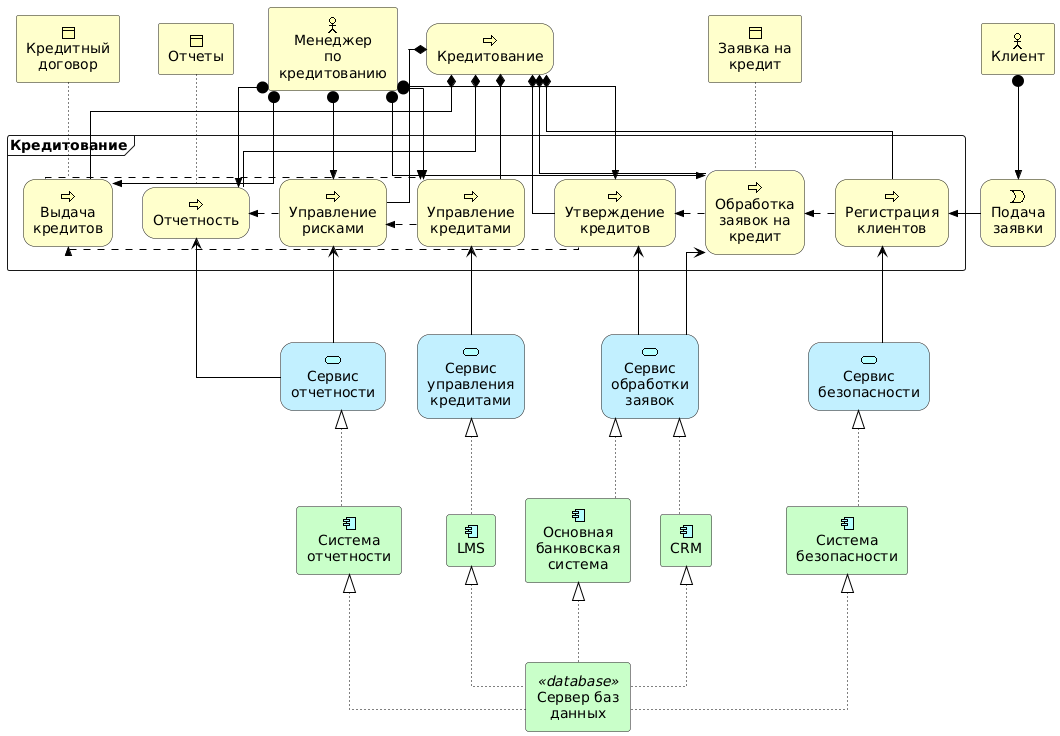
\includegraphics[width=\textwidth]{as-is-archimate.png}
	\caption{Диаграмма ArchiMate <<как есть>>}
	\label{fig:as_is_archimate}
\end{figure}

\subsection{Резюме проекта}

В этом пункте представлено резюме произведенного анализа в пунктах 1.1-1.4 и 
представлены цели и задачи сформированные в результате анализа в методике
<<SMART>> \cite{smart2.0}.

Методика <<SMART>> предназначена для определения целей выполняемых в рамках
той или иной задачи и описывает правила которым должны соответствовать цели
выполнимой задачи. Цели задачи должны быть конкретны (Specific), измеримы
(Measurable), достижимы (Achievable), релевантны (Relevant) для задачи и
ограничены по времени (Time-bounded). 

На основе анализа показателей качества обслуживания можно понять, что они
являются ниже, чем принято в мире для сектора банкинга. В первую очередь
улучшения
будут произведены для повышения технических показателей на основе которых уже
будет возможностью с легкостью улучшить бизнес показатели показатели.
Предварительно проанализировав нынешнюю ситуацию компании и определившись с
уровнем предоставления услуг другими компаниями сделан вывод, что в среднем все
технические показатели, а в частности показатели касающиеся хранения и передачи
данных должны быть улучшены на 25-30\%, что скажется на приросте бизнес
показателей, который будет составлять 20\%. Данные значения позволяют сделать
предварительные расчеты и выводы относительности стоимости и рациональности
изменений.

Оценки затрат начальных вложений в новую ИТ-инфраструктуру представлены
в Таблице \ref{tab:new-infra-coast-calc} . Внедрение и настройка представленных
компонентов составит 4.600.000 рублей, а суммарно все первоначальные вложения
обойдутся в 17.400.000 рублей.

\begin{tabularx}{\textwidth}{|l|X|X|l|}
	\captionsetup{margin=-14pt}
	\caption{Расчетная стоимость оборудования
ЦОДа\label{tab:new-infra-coast-calc}}
	\\
	\endfirsthead
	\caption*{Продолжение таблицы \ref{tab:new-infra-coast-calc}} \\
	\hline
№ & Компонент               & Описание                                        &
Затраты          \\ \hline
	\endhead
	\endfoot
	\endlastfoot
	\hline
№ & Компонент               & Описание                                        &
Затраты          \\ \hline
1 & Серверы                 & 4 высокопроизводительных                        &
3.300.000 рублей \\ \hline
2 & Система хранения        & NVMe, 100 ТБ                                    &
5.000.000 рублей \\ \hline
3 & Сетевое оборудование    & Коммутаторы и маршрутизаторы                    &
2.000.000 рублей \\
4 & Программное обеспечение & СУБД, системы безопасности, системы мониторинга &
2.500.000 рублей \\ \hline
\end{tabularx}

Годовые эксплуатационные расходы составят 4.550.000 рублей из которых 1.700.000
рублей это обслуживание и поддержка, 850.000 рублей энергопотребление,
2.000.000 рублей зарплата ИТ-персонала.

Конфигурация аппаратного обеспечения представленная выше увеличит доходы от
обработки большего числа займов. На данный момент текущая система обрабатывает
2.400 заявок в месяц, новая инфраструктура сможет обрабатывать на 20\% больше
показывая результат в 2.880 заявок в месяц, учитывая средний доход в 4500
рублей
с займа годовая выхода составит $480\;\text{заявок} \times 4.500\;\text{рублей}
\times 12\;\text{заявок} = 25.920.000\;\text{рублей}$.

Текущие простои системы составляют 10 часов в год, новые 2 часа. Стоимость
одного часа простоя 500.000 рублей, это значит, что экономия в год составит
$8\;\text{часов}\;\times\;500.000\;\text{рублей}=4.000.000\;\text{рублей}$.

Так как утечка данных является неприемлемой для сферы кредитования, средняя
стоимость утечки составляет 45.000.000 рублей. Новая инфраструктура позволит
снизить вероятность утечки данных с 10\% до 2\% в год, это означает, что
ожидаемая экономия составит $\left( 10\% - 2\%
\right)\;\times\;45.000.000\;\text{рублей}=3.600.000\;\text{в год.}$

По расчетам выше получается, что годовая выгода составит
$25.920.000+4.000.000+3.600.000=33.520.000\;\text{рублей}$. С учетом
годовых расходов на поддержание инфраструктуры в 4.550.000 рублей. Чистый
денежный
поток равен разнице между текущими расходами и новыми расходами c учетом
годовой выгоды, что составляет
$(39.480.000 - 4.550.000) + 33.520.000 = 68.450.000$ рублей в год

Расчет NPV \cite{npv} (чистая приведённая стоимость) с периодом
оценки в 5 лет и ставкой дисконтирования в 10\% годовых представлен в Формуле
\ref{eq:npv-of-improvements}.

\begin{equation} 
    \centering 
    \label{eq:npv-of-improvements}
    \begin{aligned}
        &\text{Год 1:} && \frac{68.450.000}{1 + 0.10} =
\frac{68.450.000}{1.10} = 62.227.273 \text{ рублей} \\ 
        &\text{Год 2:} && \frac{68.450.000}{(1.10)^2} =
\frac{68.450.000}{1.21} = 56.570.248 \text{ рублей} \\ 
        &\text{Год 3:} && \frac{68.450.000}{(1.10)^3} =
\frac{68.450.000}{1.331} = 51.427.498 \text{ рублей} \\ 
        &\text{Год 4:} && \frac{68.450.000}{(1.10)^4} =
\frac{68.450.000}{1.4641} = 46.752.271 \text{ рублей} \\ 
        &\text{Год 5:} && \frac{68.450.000}{(1.10)^5} =
\frac{68.450.000}{1.61051} = 42.502.065 \text{ рублей} 
    \end{aligned}
\end{equation}

Сумма приведенных денежных потоков с вычетом начальных вложений $ NPV =
-17.400.000 + 259.479.355 = 242.079.355 $ рублей. Положительное значение
показателя чистой приведенной стоимость говорит о том, что проект экономически
целесообразен.

Данная курсовая работа преследует такие цели как, разработку функциональной
модели и дизайна ИТ-инфраструктуры, которая включает в себя бизнес-слой
состоящий из таких процессов как регистрацию клиентов и обработку заявок, слой
приложения, заключающийся в CRM, LMS и основной банковской системы, и основной
технологический слой в рамках которого необходимо спланировать использование
серверов, систем хранения данных, систем передач данных и шифрования.

Наличие документации содержащей текстовое описание, диаграммы ArchiMate и DFD,
информацию об используемом системном, прикладном и аппаратном ПО, механизмов
обеспечивающих безопасное хранение данных и их быстрое перемещение в обыденном
использовании, резервном копировании и восстановлении из резервных копий,
является одной из основных целей данной дипломной работы. 

Все цели преследуемые в данной дипломной работе, которые описаны выше полностью
соответствуют методике <<SMART>>, так как они конкретны, измеряемы, достижимы,
релевантны и ограничены во времени исполнения.

В ИТ-инфраструктуре АКБ <<Абсолют Банк>> доработок и изменений преимущественно
требуют слой приложения и технологический слой, так как большинство отклонений
от желаемых SLA возникают именно по причине использования не совсем подходящих
технологий и аппаратных решений. Облачная инфраструктура в модуле
потребительского кредитования банка так же не является подходящим решением для
того количества клиентов и оборотов до которых компания доросла на данный
момент. Так же не стоит исключать и то, что компания планирует расти и набирать
обороты, а для этого ИТ-инфраструктура должна быть масштабируемой и
отказоустойчивой.


% used resources list
\begingroup
	\let\itshape\upshape
	\sloppy
	\raggedright
	\printbibliography[title=СПИСОК ИСПОЛЬЗУЕМЫХ ИСТОЧНИКОВ]
	\phantomsection
	\addcontentsline{toc}{section}{СПИСОК ИСПОЛЬЗУЕМЫХ ИСТОЧНИКОВ}
\endgroup
% used resources list

\end{document}